\begin{figure}[h!]
	\begin{center}
		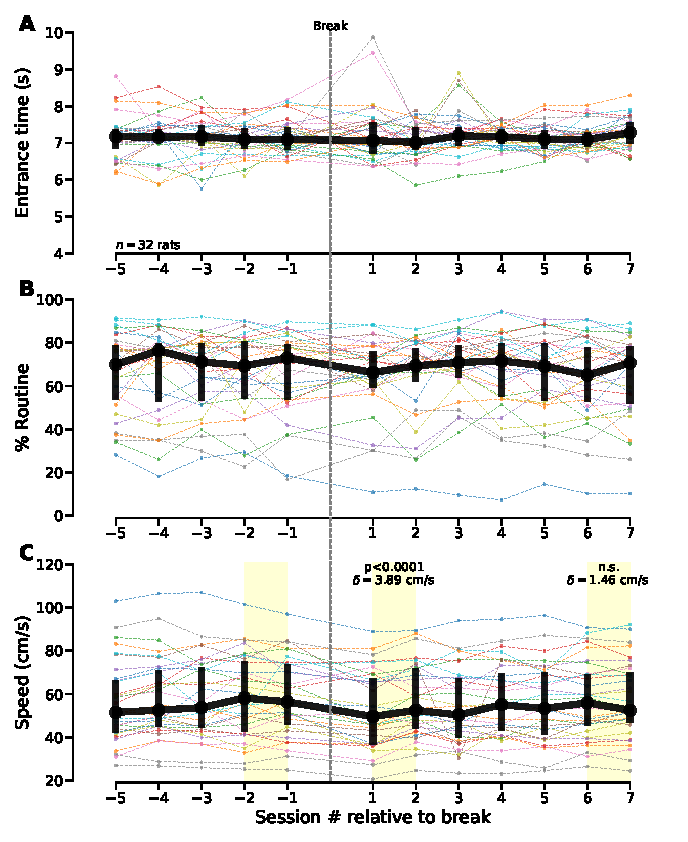
\includegraphics[scale=1]{ch-appendicies/figures/BreakEffect.pdf}
		\caption[Impact of a Two-week Break]
		{\textbf{Impact of two weeks of break on performance.}
		Task performance before and after a two week-long break in practice.
		Non-lesioned animals had stable performance before the two week-long break (same duration than lesion recovery period) in practice (\textit{A}: ET; \textit{B}: percentage of trials during which animals used the wait-and-run routine; \textit{C}: speed of the animals when they ran toward the reward area).
		A small but significant reduction in running speed was observed just after the break ($\delta$ denotes the effect size) that was restored after a few more training sessions.
		}
		\label{fig:appendix:break}
	\end{center}
\end{figure}